\documentclass{whiteboard}
\begin{document}
\begin{frame}[plain,t]
\bbcover{AIZU GRL 5A}{Diameter of a Tree}{Prof. Edson Alves}{Faculdade UnB Gama}

\end{frame}
\begin{frame}[plain,t]
\vspace*{\fill}

\bbenglish{Given a tree $T$ with non-negative weight, find the diameter of the tree.}

\vspace{0.1in}

\bbenglish{The diameter of a tree is the maximum distance between two nodes in a tree.}

\vspace*{\fill}
\end{frame}
\begin{frame}[plain,t]
\vspace*{\fill}

\bbtext{Dada uma árvore $T$ com pesos não-negativos, encontre o diâmetro desta árvore.}

\vspace{0.1in}

\bbtext{O diâmetro de uma árvore é a distância máxima entre dois vértices de uma árvore.}

\vspace*{\fill}
\end{frame}
\begin{frame}[plain,t]
\vspace*{\fill}

\bbbold{Input}

$$
\begin{array}{lll}
n \\
s_1 & t_1 & w_1 \\
s_2 & t_2 & w_2 \\
\ldots \\
s_{n-1} & t_{n-1} & w_{n-1} \\
\end{array}
$$
\vspace{0.1in}

\bbenglish{The first line consists of an integer $n$ which represents the number of nodes in the tree. Every node has a unique ID from $0$ to $n-1$ respectively.}

\vspace{0.1in}

\bbenglish{In the following $n-1$ lines, edges of the tree are given. $s_i$ and $t_i$ represent end-points of the $i$-th edge (undirected) and $w_i$ represents the weight (distance) of the $i$-th edge.}

\vspace*{\fill}
\end{frame}
\begin{frame}[plain,t]
\vspace*{\fill}

\bbbold{Entrada}

$$
\begin{array}{lll}
n \\
s_1 & t_1 & w_1 \\
s_2 & t_2 & w_2 \\
\ldots \\
s_{n-1} & t_{n-1} & w_{n-1} \\
\end{array}
$$
\vspace{0.1in}

\bbtext{A primeira linha consiste em um inteiro $n$, o qual representa o número de nós na árvore. Cada nó tem um identificador único entre $0$ e $n-1$, respectivamente.}

\vspace{0.1in}

\bbtext{Nas próximas $n-1$ linhas são dadas as arestas da árvore. $s_i$ e $t_i$ representam os pontos terminais da $i$-ésima aresta (não-direcionada) e $w_i$ representa o peso (distância) da $i$-ésima aresta.}

\vspace*{\fill}
\end{frame}
\begin{frame}[plain,t]
\vspace*{\fill}

\bbbold{Output}

\vspace{0.1in}

\bbenglish{Print the diameter of the tree in a line.}

\vspace{0.3in}

\bbbold{Constraints}

\vspace{0.1in}

\begin{itemize}
\item $1\leq n\leq 100,000$
\item $0\leq w_i\leq 1,000$
\end{itemize}

\vspace*{\fill}
\end{frame}
\begin{frame}[plain,t]
\vspace*{\fill}

\bbbold{Saída}

\vspace{0.1in}

\bbtext{Imprima, em uma linha, o diâmetro da árvore.}

\vspace{0.3in}

\bbbold{Restrições}

\vspace{0.1in}

\begin{itemize}
\item $1\leq n\leq 100,000$
\item $0\leq w_i\leq 1,000$
\end{itemize}


\vspace*{\fill}
\end{frame}
\begin{frame}[plain,t]
\begin{tikzpicture}
\node[draw,opacity=0] at (0, 0) {x};
\node[draw,opacity=0] at (14, 8) {x};

	\node[anchor=west] (header) at (0, 7.0) { \bbbold{Exemplo de entrada e saída} };

\end{tikzpicture}
\end{frame}
\begin{frame}[plain,t]
\begin{tikzpicture}
\node[draw,opacity=0] at (0, 0) {x};
\node[draw,opacity=0] at (14, 8) {x};

	\node[anchor=west] (header) at (0, 7.0) { \bbbold{Exemplo de entrada e saída} };


	\node[anchor=west] (line1) at (1.0, 6.0) { \bbtext{\texttt{4} } };

\end{tikzpicture}
\end{frame}
\begin{frame}[plain,t]
\begin{tikzpicture}
\node[draw,opacity=0] at (0, 0) {x};
\node[draw,opacity=0] at (14, 8) {x};

	\node[anchor=west] (header) at (0, 7.0) { \bbbold{Exemplo de entrada e saída} };


	\node[anchor=west] (line1) at (1.0, 6.0) { \bbtext{\texttt{4} } };


	\draw[->,color=BBViolet] (1.25, 5.0) to  (1.25, 5.75);

	\node[] (r) at (1.25, 4.75) { \footnotesize \bbcomment{\# de nós} };

\end{tikzpicture}
\end{frame}
\begin{frame}[plain,t]
\begin{tikzpicture}
\node[draw,opacity=0] at (0, 0) {x};
\node[draw,opacity=0] at (14, 8) {x};

	\node[anchor=west] (header) at (0, 7.0) { \bbbold{Exemplo de entrada e saída} };


	\node[anchor=west] (line1) at (1.0, 6.0) { \bbtext{\texttt{4} } };





	\node[draw,very thick,circle] (node0) at (7.0, 4.0) { \bbtext{0} };

	\node[draw,very thick,circle] (node1) at (10.0, 7.0) { \bbtext{1} };

	\node[draw,very thick,circle] (node2) at (13.0, 4.0) { \bbtext{2} };

	\node[draw,very thick,circle] (node3) at (10.0, 1.0) { \bbtext{3} };


\end{tikzpicture}
\end{frame}
\begin{frame}[plain,t]
\begin{tikzpicture}
\node[draw,opacity=0] at (0, 0) {x};
\node[draw,opacity=0] at (14, 8) {x};

	\node[anchor=west] (header) at (0, 7.0) { \bbbold{Exemplo de entrada e saída} };


	\node[anchor=west] (line1) at (1.0, 6.0) { \bbtext{\texttt{4} } };





	\node[draw,very thick,circle] (node0) at (7.0, 4.0) { \bbtext{0} };

	\node[draw,very thick,circle] (node1) at (10.0, 7.0) { \bbtext{1} };

	\node[draw,very thick,circle] (node2) at (13.0, 4.0) { \bbtext{2} };

	\node[draw,very thick,circle] (node3) at (10.0, 1.0) { \bbtext{3} };



	\node[anchor=west] (line2) at (1.0, 5.5) { \bbtext{\texttt{0 1 2} } };

\end{tikzpicture}
\end{frame}
\begin{frame}[plain,t]
\begin{tikzpicture}
\node[draw,opacity=0] at (0, 0) {x};
\node[draw,opacity=0] at (14, 8) {x};

	\node[anchor=west] (header) at (0, 7.0) { \bbbold{Exemplo de entrada e saída} };


	\node[anchor=west] (line1) at (1.0, 6.0) { \bbtext{\texttt{4} } };


	\draw[->,color=BBViolet] (1.25, 4.25) to  (1.25, 5.25);

	\node[] (r) at (1.25, 4.0) { \bbcomment{$u$} };


	\node[draw,very thick,circle] (node0) at (7.0, 4.0) { \bbtext{0} };

	\node[draw,very thick,circle] (node1) at (10.0, 7.0) { \bbtext{1} };

	\node[draw,very thick,circle] (node2) at (13.0, 4.0) { \bbtext{2} };

	\node[draw,very thick,circle] (node3) at (10.0, 1.0) { \bbtext{3} };



	\node[anchor=west] (line2) at (1.0, 5.5) { \bbtext{\texttt{0 1 2} } };



\end{tikzpicture}
\end{frame}
\begin{frame}[plain,t]
\begin{tikzpicture}
\node[draw,opacity=0] at (0, 0) {x};
\node[draw,opacity=0] at (14, 8) {x};

	\node[anchor=west] (header) at (0, 7.0) { \bbbold{Exemplo de entrada e saída} };


	\node[anchor=west] (line1) at (1.0, 6.0) { \bbtext{\texttt{4} } };


	\draw[->,color=BBViolet] (1.65, 4.25) to  (1.65, 5.25);

	\node[] (r) at (1.65, 4.0) { \bbcomment{$v$} };


	\node[draw,very thick,circle] (node0) at (7.0, 4.0) { \bbtext{0} };

	\node[draw,very thick,circle] (node1) at (10.0, 7.0) { \bbtext{1} };

	\node[draw,very thick,circle] (node2) at (13.0, 4.0) { \bbtext{2} };

	\node[draw,very thick,circle] (node3) at (10.0, 1.0) { \bbtext{3} };



	\node[anchor=west] (line2) at (1.0, 5.5) { \bbtext{\texttt{0 1 2} } };





\end{tikzpicture}
\end{frame}
\begin{frame}[plain,t]
\begin{tikzpicture}
\node[draw,opacity=0] at (0, 0) {x};
\node[draw,opacity=0] at (14, 8) {x};

	\node[anchor=west] (header) at (0, 7.0) { \bbbold{Exemplo de entrada e saída} };


	\node[anchor=west] (line1) at (1.0, 6.0) { \bbtext{\texttt{4} } };


	\draw[->,color=BBViolet] (2.05, 4.25) to  (2.05, 5.25);

	\node[] (r) at (2.05, 4.0) { \bbcomment{$w$} };


	\node[draw,very thick,circle] (node0) at (7.0, 4.0) { \bbtext{0} };

	\node[draw,very thick,circle] (node1) at (10.0, 7.0) { \bbtext{1} };

	\node[draw,very thick,circle] (node2) at (13.0, 4.0) { \bbtext{2} };

	\node[draw,very thick,circle] (node3) at (10.0, 1.0) { \bbtext{3} };



	\node[anchor=west] (line2) at (1.0, 5.5) { \bbtext{\texttt{0 1 2} } };







\end{tikzpicture}
\end{frame}
\begin{frame}[plain,t]
\begin{tikzpicture}
\node[draw,opacity=0] at (0, 0) {x};
\node[draw,opacity=0] at (14, 8) {x};

	\node[anchor=west] (header) at (0, 7.0) { \bbbold{Exemplo de entrada e saída} };


	\node[anchor=west] (line1) at (1.0, 6.0) { \bbtext{\texttt{4} } };





	\node[draw,very thick,circle] (node0) at (7.0, 4.0) { \bbtext{0} };

	\node[draw,very thick,circle] (node1) at (10.0, 7.0) { \bbtext{1} };

	\node[draw,very thick,circle] (node2) at (13.0, 4.0) { \bbtext{2} };

	\node[draw,very thick,circle] (node3) at (10.0, 1.0) { \bbtext{3} };



	\node[anchor=west] (line2) at (1.0, 5.5) { \bbtext{\texttt{0 1 2} } };









	\draw[very thick](node0) to node[above left] { \bbinfo{2} } (node1);

\end{tikzpicture}
\end{frame}
\begin{frame}[plain,t]
\begin{tikzpicture}
\node[draw,opacity=0] at (0, 0) {x};
\node[draw,opacity=0] at (14, 8) {x};

	\node[anchor=west] (header) at (0, 7.0) { \bbbold{Exemplo de entrada e saída} };


	\node[anchor=west] (line1) at (1.0, 6.0) { \bbtext{\texttt{4} } };





	\node[draw,very thick,circle] (node0) at (7.0, 4.0) { \bbtext{0} };

	\node[draw,very thick,circle] (node1) at (10.0, 7.0) { \bbtext{1} };

	\node[draw,very thick,circle] (node2) at (13.0, 4.0) { \bbtext{2} };

	\node[draw,very thick,circle] (node3) at (10.0, 1.0) { \bbtext{3} };



	\node[anchor=west] (line2) at (1.0, 5.5) { \bbtext{\texttt{0 1 2} } };









	\draw[very thick](node0) to node[above left] { \bbinfo{2} } (node1);


	\node[anchor=west] (line3) at (1.0, 5.0) { \bbtext{\texttt{1 2 1} } };

\end{tikzpicture}
\end{frame}
\begin{frame}[plain,t]
\begin{tikzpicture}
\node[draw,opacity=0] at (0, 0) {x};
\node[draw,opacity=0] at (14, 8) {x};

	\node[anchor=west] (header) at (0, 7.0) { \bbbold{Exemplo de entrada e saída} };


	\node[anchor=west] (line1) at (1.0, 6.0) { \bbtext{\texttt{4} } };





	\node[draw,very thick,circle] (node0) at (7.0, 4.0) { \bbtext{0} };

	\node[draw,very thick,circle] (node1) at (10.0, 7.0) { \bbtext{1} };

	\node[draw,very thick,circle] (node2) at (13.0, 4.0) { \bbtext{2} };

	\node[draw,very thick,circle] (node3) at (10.0, 1.0) { \bbtext{3} };



	\node[anchor=west] (line2) at (1.0, 5.5) { \bbtext{\texttt{0 1 2} } };









	\draw[very thick](node0) to node[above left] { \bbinfo{2} } (node1);


	\node[anchor=west] (line3) at (1.0, 5.0) { \bbtext{\texttt{1 2 1} } };


	\draw[very thick](node2) to node[above right] { \bbinfo{1} } (node1);


\end{tikzpicture}
\end{frame}
\begin{frame}[plain,t]
\begin{tikzpicture}
\node[draw,opacity=0] at (0, 0) {x};
\node[draw,opacity=0] at (14, 8) {x};

	\node[anchor=west] (header) at (0, 7.0) { \bbbold{Exemplo de entrada e saída} };


	\node[anchor=west] (line1) at (1.0, 6.0) { \bbtext{\texttt{4} } };





	\node[draw,very thick,circle] (node0) at (7.0, 4.0) { \bbtext{0} };

	\node[draw,very thick,circle] (node1) at (10.0, 7.0) { \bbtext{1} };

	\node[draw,very thick,circle] (node2) at (13.0, 4.0) { \bbtext{2} };

	\node[draw,very thick,circle] (node3) at (10.0, 1.0) { \bbtext{3} };



	\node[anchor=west] (line2) at (1.0, 5.5) { \bbtext{\texttt{0 1 2} } };









	\draw[very thick](node0) to node[above left] { \bbinfo{2} } (node1);


	\node[anchor=west] (line3) at (1.0, 5.0) { \bbtext{\texttt{1 2 1} } };


	\draw[very thick](node2) to node[above right] { \bbinfo{1} } (node1);



	\node[anchor=west] (line4) at (1.0, 4.5) { \bbtext{\texttt{1 3 3} } };

\end{tikzpicture}
\end{frame}
\begin{frame}[plain,t]
\begin{tikzpicture}
\node[draw,opacity=0] at (0, 0) {x};
\node[draw,opacity=0] at (14, 8) {x};

	\node[anchor=west] (header) at (0, 7.0) { \bbbold{Exemplo de entrada e saída} };


	\node[anchor=west] (line1) at (1.0, 6.0) { \bbtext{\texttt{4} } };





	\node[draw,very thick,circle] (node0) at (7.0, 4.0) { \bbtext{0} };

	\node[draw,very thick,circle] (node1) at (10.0, 7.0) { \bbtext{1} };

	\node[draw,very thick,circle] (node2) at (13.0, 4.0) { \bbtext{2} };

	\node[draw,very thick,circle] (node3) at (10.0, 1.0) { \bbtext{3} };



	\node[anchor=west] (line2) at (1.0, 5.5) { \bbtext{\texttt{0 1 2} } };









	\draw[very thick](node0) to node[above left] { \bbinfo{2} } (node1);


	\node[anchor=west] (line3) at (1.0, 5.0) { \bbtext{\texttt{1 2 1} } };


	\draw[very thick](node2) to node[above right] { \bbinfo{1} } (node1);



	\node[anchor=west] (line4) at (1.0, 4.5) { \bbtext{\texttt{1 3 3} } };


	\draw[very thick](node3) to node[right] { \bbinfo{3} } (node1);

\end{tikzpicture}
\end{frame}
\begin{frame}[plain,t]
\begin{tikzpicture}
\node[draw,opacity=0] at (0, 0) {x};
\node[draw,opacity=0] at (14, 8) {x};

	\node[anchor=west] (header) at (0, 7.0) { \bbbold{Exemplo de entrada e saída} };


	\node[anchor=west] (line1) at (1.0, 6.0) { \bbtext{\texttt{4} } };





	\node[draw,very thick,circle] (node0) at (7.0, 4.0) { \bbtext{0} };

	\node[draw,very thick,circle] (node1) at (10.0, 7.0) { \bbtext{1} };

	\node[draw,very thick,circle] (node2) at (13.0, 4.0) { \bbtext{2} };

	\node[draw,very thick,circle] (node3) at (10.0, 1.0) { \bbtext{3} };



	\node[anchor=west] (line2) at (1.0, 5.5) { \bbtext{\texttt{0 1 2} } };









	\draw[very thick,color=BBCyan,dashed](node0) to node[above left] { \bbinfo{2} } (node1);


	\node[anchor=west] (line3) at (1.0, 5.0) { \bbtext{\texttt{1 2 1} } };


	\draw[very thick](node2) to node[above right] { \bbinfo{1} } (node1);



	\node[anchor=west] (line4) at (1.0, 4.5) { \bbtext{\texttt{1 3 3} } };


	\draw[very thick,color=BBCyan,dashed](node3) to node[right] { \bbinfo{3} } (node1);


\end{tikzpicture}
\end{frame}
\begin{frame}[plain,t]
\begin{tikzpicture}
\node[draw,opacity=0] at (0, 0) {x};
\node[draw,opacity=0] at (14, 8) {x};

	\node[anchor=west] (header) at (0, 7.0) { \bbbold{Exemplo de entrada e saída} };


	\node[anchor=west] (line1) at (1.0, 6.0) { \bbtext{\texttt{4} } };


	\draw[->,color=BBBlack,thick,-latex] (1.65, 4.25) to  (1.65, 3.25);

	\node[] (r) at (1.65, 3.0) { \bboutput{2 + 3 = 5} };


	\node[draw,very thick,circle] (node0) at (7.0, 4.0) { \bbtext{0} };

	\node[draw,very thick,circle] (node1) at (10.0, 7.0) { \bbtext{1} };

	\node[draw,very thick,circle] (node2) at (13.0, 4.0) { \bbtext{2} };

	\node[draw,very thick,circle] (node3) at (10.0, 1.0) { \bbtext{3} };



	\node[anchor=west] (line2) at (1.0, 5.5) { \bbtext{\texttt{0 1 2} } };









	\draw[very thick,color=BBCyan,dashed](node0) to node[above left] { \bbinfo{2} } (node1);


	\node[anchor=west] (line3) at (1.0, 5.0) { \bbtext{\texttt{1 2 1} } };


	\draw[very thick](node2) to node[above right] { \bbinfo{1} } (node1);



	\node[anchor=west] (line4) at (1.0, 4.5) { \bbtext{\texttt{1 3 3} } };


	\draw[very thick,color=BBCyan,dashed](node3) to node[right] { \bbinfo{3} } (node1);




\end{tikzpicture}
\end{frame}
\begin{frame}[plain,t]
\begin{tikzpicture}
\node[draw,opacity=0] at (0, 0) {x};
\node[draw,opacity=0] at (14, 8) {x};

	\node[anchor=west] (header) at (0, 7.0) { \bbbold{Exemplo de entrada e saída} };

\end{tikzpicture}
\end{frame}
\begin{frame}[plain,t]
\begin{tikzpicture}
\node[draw,opacity=0] at (0, 0) {x};
\node[draw,opacity=0] at (14, 8) {x};

	\node[anchor=west] (header) at (0, 7.0) { \bbbold{Exemplo de entrada e saída} };


	\node[anchor=west] (line1) at (1.0, 6.0) { \bbtext{\texttt{4} } };




\end{tikzpicture}
\end{frame}
\begin{frame}[plain,t]
\begin{tikzpicture}
\node[draw,opacity=0] at (0, 0) {x};
\node[draw,opacity=0] at (14, 8) {x};

	\node[anchor=west] (header) at (0, 7.0) { \bbbold{Exemplo de entrada e saída} };


	\node[anchor=west] (line1) at (1.0, 6.0) { \bbtext{\texttt{4} } };





	\node[draw,very thick,circle] (node0) at (7.0, 4.0) { \bbtext{0} };

	\node[draw,very thick,circle] (node1) at (10.0, 7.0) { \bbtext{1} };

	\node[draw,very thick,circle] (node2) at (13.0, 4.0) { \bbtext{2} };

	\node[draw,very thick,circle] (node3) at (10.0, 1.0) { \bbtext{3} };


\end{tikzpicture}
\end{frame}
\begin{frame}[plain,t]
\begin{tikzpicture}
\node[draw,opacity=0] at (0, 0) {x};
\node[draw,opacity=0] at (14, 8) {x};

	\node[anchor=west] (header) at (0, 7.0) { \bbbold{Exemplo de entrada e saída} };


	\node[anchor=west] (line1) at (1.0, 6.0) { \bbtext{\texttt{4} } };





	\node[draw,very thick,circle] (node0) at (7.0, 4.0) { \bbtext{0} };

	\node[draw,very thick,circle] (node1) at (10.0, 7.0) { \bbtext{1} };

	\node[draw,very thick,circle] (node2) at (13.0, 4.0) { \bbtext{2} };

	\node[draw,very thick,circle] (node3) at (10.0, 1.0) { \bbtext{3} };



	\node[anchor=west] (line2) at (1.0, 5.5) { \bbtext{\texttt{0 1 1} } };

\end{tikzpicture}
\end{frame}
\begin{frame}[plain,t]
\begin{tikzpicture}
\node[draw,opacity=0] at (0, 0) {x};
\node[draw,opacity=0] at (14, 8) {x};

	\node[anchor=west] (header) at (0, 7.0) { \bbbold{Exemplo de entrada e saída} };


	\node[anchor=west] (line1) at (1.0, 6.0) { \bbtext{\texttt{4} } };





	\node[draw,very thick,circle] (node0) at (7.0, 4.0) { \bbtext{0} };

	\node[draw,very thick,circle] (node1) at (10.0, 7.0) { \bbtext{1} };

	\node[draw,very thick,circle] (node2) at (13.0, 4.0) { \bbtext{2} };

	\node[draw,very thick,circle] (node3) at (10.0, 1.0) { \bbtext{3} };



	\node[anchor=west] (line2) at (1.0, 5.5) { \bbtext{\texttt{0 1 1} } };


	\draw[very thick](node0) to node[above left] { \bbinfo{1} } (node1);

\end{tikzpicture}
\end{frame}
\begin{frame}[plain,t]
\begin{tikzpicture}
\node[draw,opacity=0] at (0, 0) {x};
\node[draw,opacity=0] at (14, 8) {x};

	\node[anchor=west] (header) at (0, 7.0) { \bbbold{Exemplo de entrada e saída} };


	\node[anchor=west] (line1) at (1.0, 6.0) { \bbtext{\texttt{4} } };





	\node[draw,very thick,circle] (node0) at (7.0, 4.0) { \bbtext{0} };

	\node[draw,very thick,circle] (node1) at (10.0, 7.0) { \bbtext{1} };

	\node[draw,very thick,circle] (node2) at (13.0, 4.0) { \bbtext{2} };

	\node[draw,very thick,circle] (node3) at (10.0, 1.0) { \bbtext{3} };



	\node[anchor=west] (line2) at (1.0, 5.5) { \bbtext{\texttt{0 1 1} } };


	\draw[very thick](node0) to node[above left] { \bbinfo{1} } (node1);


	\node[anchor=west] (line3) at (1.0, 5.0) { \bbtext{\texttt{1 2 2} } };

\end{tikzpicture}
\end{frame}
\begin{frame}[plain,t]
\begin{tikzpicture}
\node[draw,opacity=0] at (0, 0) {x};
\node[draw,opacity=0] at (14, 8) {x};

	\node[anchor=west] (header) at (0, 7.0) { \bbbold{Exemplo de entrada e saída} };


	\node[anchor=west] (line1) at (1.0, 6.0) { \bbtext{\texttt{4} } };





	\node[draw,very thick,circle] (node0) at (7.0, 4.0) { \bbtext{0} };

	\node[draw,very thick,circle] (node1) at (10.0, 7.0) { \bbtext{1} };

	\node[draw,very thick,circle] (node2) at (13.0, 4.0) { \bbtext{2} };

	\node[draw,very thick,circle] (node3) at (10.0, 1.0) { \bbtext{3} };



	\node[anchor=west] (line2) at (1.0, 5.5) { \bbtext{\texttt{0 1 1} } };


	\draw[very thick](node0) to node[above left] { \bbinfo{1} } (node1);


	\node[anchor=west] (line3) at (1.0, 5.0) { \bbtext{\texttt{1 2 2} } };


	\draw[very thick](node2) to node[above right] { \bbinfo{2} } (node1);


\end{tikzpicture}
\end{frame}
\begin{frame}[plain,t]
\begin{tikzpicture}
\node[draw,opacity=0] at (0, 0) {x};
\node[draw,opacity=0] at (14, 8) {x};

	\node[anchor=west] (header) at (0, 7.0) { \bbbold{Exemplo de entrada e saída} };


	\node[anchor=west] (line1) at (1.0, 6.0) { \bbtext{\texttt{4} } };





	\node[draw,very thick,circle] (node0) at (7.0, 4.0) { \bbtext{0} };

	\node[draw,very thick,circle] (node1) at (10.0, 7.0) { \bbtext{1} };

	\node[draw,very thick,circle] (node2) at (13.0, 4.0) { \bbtext{2} };

	\node[draw,very thick,circle] (node3) at (10.0, 1.0) { \bbtext{3} };



	\node[anchor=west] (line2) at (1.0, 5.5) { \bbtext{\texttt{0 1 1} } };


	\draw[very thick](node0) to node[above left] { \bbinfo{1} } (node1);


	\node[anchor=west] (line3) at (1.0, 5.0) { \bbtext{\texttt{1 2 2} } };


	\draw[very thick](node2) to node[above right] { \bbinfo{2} } (node1);



	\node[anchor=west] (line4) at (1.0, 4.5) { \bbtext{\texttt{2 3 4} } };

\end{tikzpicture}
\end{frame}
\begin{frame}[plain,t]
\begin{tikzpicture}
\node[draw,opacity=0] at (0, 0) {x};
\node[draw,opacity=0] at (14, 8) {x};

	\node[anchor=west] (header) at (0, 7.0) { \bbbold{Exemplo de entrada e saída} };


	\node[anchor=west] (line1) at (1.0, 6.0) { \bbtext{\texttt{4} } };





	\node[draw,very thick,circle] (node0) at (7.0, 4.0) { \bbtext{0} };

	\node[draw,very thick,circle] (node1) at (10.0, 7.0) { \bbtext{1} };

	\node[draw,very thick,circle] (node2) at (13.0, 4.0) { \bbtext{2} };

	\node[draw,very thick,circle] (node3) at (10.0, 1.0) { \bbtext{3} };



	\node[anchor=west] (line2) at (1.0, 5.5) { \bbtext{\texttt{0 1 1} } };


	\draw[very thick](node0) to node[above left] { \bbinfo{1} } (node1);


	\node[anchor=west] (line3) at (1.0, 5.0) { \bbtext{\texttt{1 2 2} } };


	\draw[very thick](node2) to node[above right] { \bbinfo{2} } (node1);



	\node[anchor=west] (line4) at (1.0, 4.5) { \bbtext{\texttt{2 3 4} } };


	\draw[very thick](node3) to node[below right] { \bbinfo{4} } (node2);

\end{tikzpicture}
\end{frame}
\begin{frame}[plain,t]
\begin{tikzpicture}
\node[draw,opacity=0] at (0, 0) {x};
\node[draw,opacity=0] at (14, 8) {x};

	\node[anchor=west] (header) at (0, 7.0) { \bbbold{Exemplo de entrada e saída} };


	\node[anchor=west] (line1) at (1.0, 6.0) { \bbtext{\texttt{4} } };





	\node[draw,very thick,circle] (node0) at (7.0, 4.0) { \bbtext{0} };

	\node[draw,very thick,circle] (node1) at (10.0, 7.0) { \bbtext{1} };

	\node[draw,very thick,circle] (node2) at (13.0, 4.0) { \bbtext{2} };

	\node[draw,very thick,circle] (node3) at (10.0, 1.0) { \bbtext{3} };



	\node[anchor=west] (line2) at (1.0, 5.5) { \bbtext{\texttt{0 1 1} } };


	\draw[very thick,color=BBCyan,dashed](node0) to node[above left] { \bbinfo{1} } (node1);


	\node[anchor=west] (line3) at (1.0, 5.0) { \bbtext{\texttt{1 2 2} } };


	\draw[very thick,color=BBCyan,dashed](node2) to node[above right] { \bbinfo{2} } (node1);



	\node[anchor=west] (line4) at (1.0, 4.5) { \bbtext{\texttt{2 3 4} } };


	\draw[very thick,color=BBCyan,dashed](node3) to node[below right] { \bbinfo{4} } (node2);


\end{tikzpicture}
\end{frame}
\begin{frame}[plain,t]
\begin{tikzpicture}
\node[draw,opacity=0] at (0, 0) {x};
\node[draw,opacity=0] at (14, 8) {x};

	\node[anchor=west] (header) at (0, 7.0) { \bbbold{Exemplo de entrada e saída} };


	\node[anchor=west] (line1) at (1.0, 6.0) { \bbtext{\texttt{4} } };

	\draw[->,color=BBBlack,thick,-latex] (1.65, 4.25) to  (1.65, 3.25);

	\node[] (r) at (1.65, 3.0) { \bboutput{1 + 2 + 4 = 7} };



	\node[draw,very thick,circle] (node0) at (7.0, 4.0) { \bbtext{0} };

	\node[draw,very thick,circle] (node1) at (10.0, 7.0) { \bbtext{1} };

	\node[draw,very thick,circle] (node2) at (13.0, 4.0) { \bbtext{2} };

	\node[draw,very thick,circle] (node3) at (10.0, 1.0) { \bbtext{3} };



	\node[anchor=west] (line2) at (1.0, 5.5) { \bbtext{\texttt{0 1 1} } };


	\draw[very thick,color=BBCyan,dashed](node0) to node[above left] { \bbinfo{1} } (node1);


	\node[anchor=west] (line3) at (1.0, 5.0) { \bbtext{\texttt{1 2 2} } };


	\draw[very thick,color=BBCyan,dashed](node2) to node[above right] { \bbinfo{2} } (node1);



	\node[anchor=west] (line4) at (1.0, 4.5) { \bbtext{\texttt{2 3 4} } };


	\draw[very thick,color=BBCyan,dashed](node3) to node[below right] { \bbinfo{4} } (node2);




\end{tikzpicture}
\end{frame}
\begin{frame}[plain,t]
\begin{tikzpicture}
\node[draw,opacity=0] at (0, 0) {x};
\node[draw,opacity=0] at (14, 8) {x};

	\node[anchor=west] (header) at (0.0, 6.0) { \Large \bbbold{Solução} };

\end{tikzpicture}
\end{frame}
\begin{frame}[plain,t]
\begin{tikzpicture}
\node[draw,opacity=0] at (0, 0) {x};
\node[draw,opacity=0] at (14, 8) {x};

	\node[anchor=west] (header) at (0.0, 6.0) { \Large \bbbold{Solução} };


	\node[anchor=west] (line1) at (1.0, 5.0) { $\star$ \bbtext{O diâmetro também pode ser computado por meio de duas DFS} };

\end{tikzpicture}
\end{frame}
\begin{frame}[plain,t]
\begin{tikzpicture}
\node[draw,opacity=0] at (0, 0) {x};
\node[draw,opacity=0] at (14, 8) {x};

	\node[anchor=west] (header) at (0.0, 6.0) { \Large \bbbold{Solução} };


	\node[anchor=west] (line1) at (1.0, 5.0) { $\star$ \bbtext{O diâmetro também pode ser computado por meio de duas DFS} };


	\node[anchor=west] (line11) at (1.0, 4.0) { $\star$ \bbtext{Isto porque, em árvores, todos caminhos mínimos são únicos} };

\end{tikzpicture}
\end{frame}
\begin{frame}[plain,t]
\begin{tikzpicture}
\node[draw,opacity=0] at (0, 0) {x};
\node[draw,opacity=0] at (14, 8) {x};

	\node[anchor=west] (header) at (0.0, 6.0) { \Large \bbbold{Solução} };


	\node[anchor=west] (line1) at (1.0, 5.0) { $\star$ \bbtext{O diâmetro também pode ser computado por meio de duas DFS} };


	\node[anchor=west] (line11) at (1.0, 4.0) { $\star$ \bbtext{Isto porque, em árvores, todos caminhos mínimos são únicos} };


	\node[anchor=west] (line2) at (1.0, 3.0) { $\star$ \bbtext{A DFS encurta o código} };

\end{tikzpicture}
\end{frame}
\begin{frame}[plain,t]
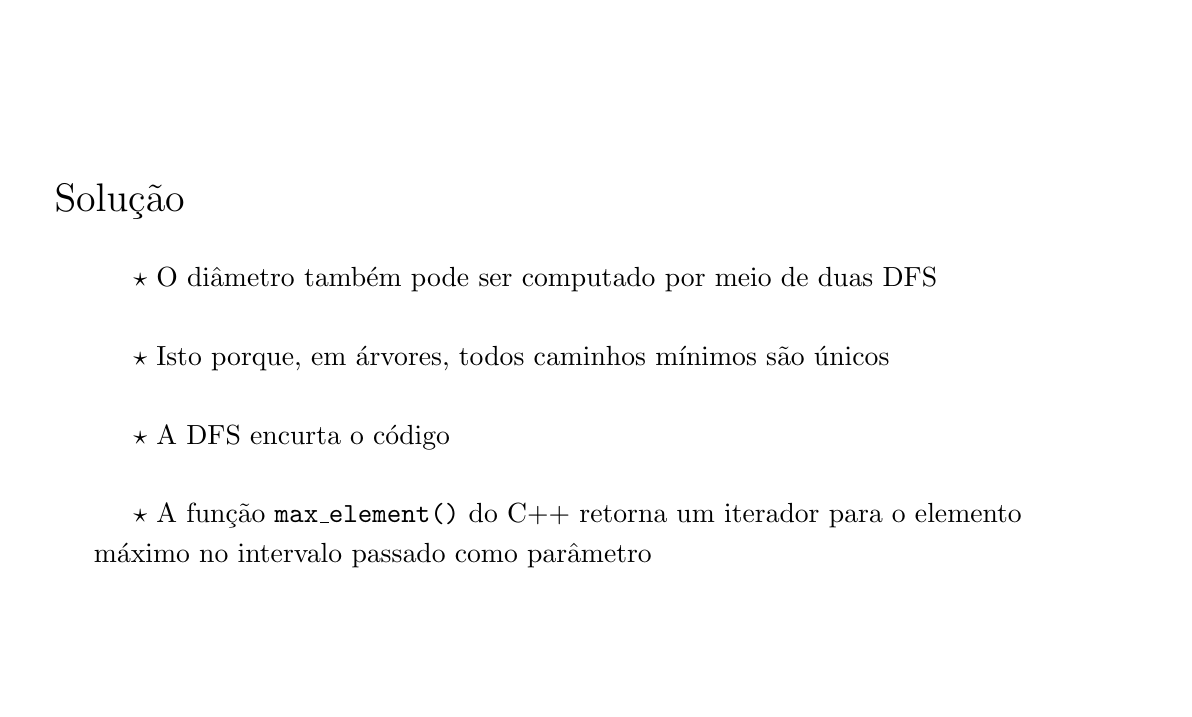
\begin{tikzpicture}
\node[draw,opacity=0] at (0, 0) {x};
\node[draw,opacity=0] at (14, 8) {x};

	\node[anchor=west] (header) at (0.0, 6.0) { \Large \bbbold{Solução} };


	\node[anchor=west] (line1) at (1.0, 5.0) { $\star$ \bbtext{O diâmetro também pode ser computado por meio de duas DFS} };


	\node[anchor=west] (line11) at (1.0, 4.0) { $\star$ \bbtext{Isto porque, em árvores, todos caminhos mínimos são únicos} };


	\node[anchor=west] (line2) at (1.0, 3.0) { $\star$ \bbtext{A DFS encurta o código} };


	\node[anchor=west] (line3) at (1.0, 2.0) { $\star$ \bbtext{A função \texttt{max\_element()} do C++ retorna um iterador para o elemento} };

	\node[anchor=west] (line31) at (0.5, 1.5) { \bbtext{máximo no intervalo passado como parâmetro} };

\end{tikzpicture}
\end{frame}
\begin{frame}[plain,t]

\inputsnippet{cpp}{10}{20}{codes/GRL_5_A.cpp}

\end{frame}
\begin{frame}[plain,t]

\inputsnippet{cpp}{22}{35}{codes/GRL_5_A.cpp}

\end{frame}
\end{document}
